\documentclass[pt12]{beamer}
%\documentclass[pt12,externalviewer]{beamer}

\usepackage{amssymb}
\usepackage{minted}
%\usepackage{rotating}
%\usepackage{amsmath}
\usepackage{tikz}
\newcommand\encircle[1]{%
	\tikz[baseline=(X.base)] 
	\node (X) [draw, shape=circle, inner sep=0] {\strut #1};}
%\usepackage{beamergraphics}
\usepackage[latin1]{inputenc}
\usepackage[T1]{fontenc}
\usepackage{multicol}
\usepackage{svg}
%\usepackage[absolute,overlay]{textpos}
%\usepackage{pdfcolparallel}

%\usepackage{tcolorbox}
%\tcbuselibrary{fitting}

\definecolor{PDred}{HTML}{9A001B}

\mode<presentation>
{
  \usetheme{Warsaw} 
%  \usetheme{Madrid}
%  \usetheme{Montpellier}
%  \usetheme{Marburg} 
  \usecolortheme[named=PDred]{structure}
  \setbeamercolor{alerted text}{fg=PDred}
  \setbeamercovered{transparent}
  \setbeamertemplate{section in toc}[ball unnumbered]
}

%\setbeamertemplate{footline}{\hfill\insertframenumber/\inserttotalframenumber} 

\expandafter\def\expandafter\insertshorttitle\expandafter{%
  \insertshorttitle\hfill%
  \insertframenumber\,/\,\inserttotalframenumber}

\newcommand{\backupbegin}{
   \newcounter{framenumberappendix}
   \setcounter{framenumberappendix}{\value{framenumber}}
}
\newcommand{\backupend}{
   \addtocounter{framenumberappendix}{-\value{framenumber}}
   \addtocounter{framenumber}{\value{framenumberappendix}} 
}

\newcommand{\refer}[1]{%
   \begin{flushright}
      {\alert{\tiny #1}}
   \end{flushright}}
  
\newcommand{\lrefer}[1]{%
   \begin{flushleft}
      {\alert{\tiny #1}}
   \end{flushleft}}
  
\newcommand{\param}[1]{%
   \begin{flushright}
      {\small #1}
   \end{flushright}
   \vspace{-1.5\baselineskip}
}

\newcommand{\sech}{\mathop{\rm sech}\nolimits}
\newcommand{\sgn}{\mathop{\rm sgn}\nolimits}
\newcommand{\etal}{{\em et al.}}


\title[Renormalization Group]{Renormalization Group}

\author[Saverio Monaco]{\large{Saverio Monaco}\bigskip\\ Quantum Information and Computing}
\date{\today}
\institute[DFA.UniCT]{
\begin{minipage}[c]{1.3truecm}

\includegraphics[width=\textwidth]{../../teximgs/PODlogo}
\end{minipage}
\begin{minipage}[c]{4.7truecm}
\begin{flushleft}
\begin{sl}
Dipartimento di Fisica e Astronomia\\ 
``Galileo Galilei''
\end{sl}
\end{flushleft}
\end{minipage}
\begin{minipage}[c]{3.2truecm}

\includegraphics[width=\textwidth]{../../teximgs/800anni_logo}
\end{minipage}}


\begin{document}

\begin{frame}[plain]
\titlepage
\end{frame}

\newcommand{\ket}[1]{\left|#1\right>}
\newcommand{\bra}[1]{\left<#1\right|}

\begin{frame}[label=Theory]
\frametitle{Theory}
\tableofcontents[pausesections]
\textbf{1-D Ising Model:}
\begin{center}
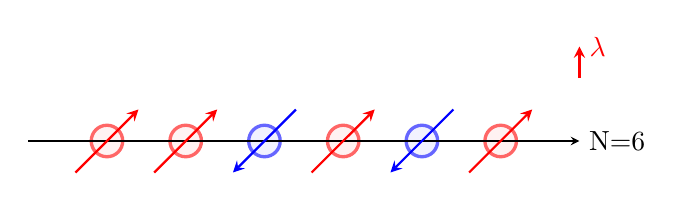
\begin{tikzpicture}
	\filldraw[color=red!60, fill=red!5, very thick](0,0) circle (.2);
	\filldraw[color=red!60, fill=red!5, very thick](1,0) circle (.2);
	\filldraw[color=blue!60, fill=blue!5, very thick](2,0) circle (.2);
	\filldraw[color=red!60, fill=red!5, very thick](3,0) circle (.2);
	\filldraw[color=blue!60, fill=blue!5, very thick](4,0) circle (.2);
	\filldraw[color=red!60, fill=red!5, very thick](5,0) circle (.2);
	\draw [-stealth](-1,0) -- (6,0)node[anchor=west]{N=6};
	\draw [-stealth,color=red, thick](-.4,-.4) -- (.4,.4);
	\draw [-stealth,color=red, thick](1-.4,-.4) -- (1+.4,.4);
	\draw [-stealth,color=blue, thick](2+.4,+.4) -- (2-.4,-.4);
	\draw [-stealth,color=red, thick](3-.4,-.4) -- (3+.4,.4);
	\draw [-stealth,color=blue, thick](4+.4,+.4) -- (4-.4,-.4);
	\draw [-stealth,color=red, thick](5-.4,-.4) -- (5+.4,.4);
	
	\draw [-stealth,color=red,thick](6,.8) -- (6,1.2)node[anchor=west]{$\lambda$};
\end{tikzpicture}
\end{center}
\begin{equation*}
	H = {\lambda\sum_i^N \sigma_z^i}-{\sum_i^{N-1}\sigma_x^{i+1}\sigma_x^i}
\end{equation*}
where
\begin{equation*}
	\sigma_z^i = \underbrace{\mathbb{I}\otimes\mathbb{I}\otimes...\otimes\mathbb{I}}_{i-1}\otimes\begin{pmatrix}
		1 & 0 \\ 0 & -1
	\end{pmatrix}\otimes\underbrace{\mathbb{I}\otimes...\otimes\mathbb{I}}_{N-i}
\end{equation*}
\begin{equation*}
	\sigma_x^i = \underbrace{\mathbb{I}\otimes\mathbb{I}\otimes...\otimes\mathbb{I}}_{i-1}\otimes\begin{pmatrix}
		0 & 1 \\ 1 & 0
	\end{pmatrix}\otimes\underbrace{\mathbb{I}\otimes...\otimes\mathbb{I}}_{N-i}
\end{equation*}
\end{frame}

\begin{frame}[fragile,label=RB]
	\frametitle{Renormalization Group algorithm}
	\tableofcontents[pausesections]
	\textbf{Algorithm:}
	\begin{itemize}
		\item[\textbf{1.}] Initialize Ising's Hamiltonian for a given N:  $H_N$
		\item[\textbf{2.}] Double the system size:
		$$
		\begin{align}
			H_{2N} &= H^{L}_N + H^R_N + H^{INT} =\\
			       &= H_N\otimes \bigotimes_{i=1}^{N}\mathbb{I} + \bigotimes_{i=1}^{N}\mathbb{I} \otimes H_N
		\end{align}$$ 
	\end{itemize}
\end{frame}

\begin{frame}[fragile,label=RB]
	\frametitle{Renormalization Group}
	\tableofcontents[pausesections]
\end{frame}

\include{sslide}

\end{document}

